\chapter{Rendre \vim utilisable}

\newthought{Ça peut paraître étonnant} comme approche, mais c'est pour moi la première chose à faire : rendre \vim utilisable par un humain lambda. Si tout le monde semble s'accorder sur le fait que \vim est un \textbf{éditeur très puissant}, tout le monde pourra aussi s'accorder sur le fait que de base, il est totalement \textbf{imbitable}. Soyons honnête, sans une configuration par défaut minimale, utiliser \vim est \textbf{contre-productif}. 

C'est à mon avis le premier obstacle à surmonter avant toute autre chose. C'est ce que les autres éditeurs « à la mode » comme Textmate, Sublimetext, Notepad++ ou Netbeans proposent, c'est à dire un environnement à minima utilisable tel quel, même si l'on en n'exploite pas la totalité.

Voici donc ce qui manque à un \vim nu (et ce qui est pour moi une \textbf{cause d'abandon pour beaucoup} d'entre vous) :

\begin{marginfigure}%
  
\includegraphics[width=\linewidth]{solarized-yinyang.png}
  \caption{Le thème \emph{Solarized} en sombre et en clair. \url{http://ethanschoonover.com/solarized}}
  \label{fig:solarized}
\end{marginfigure}

\begin{description}
    \item[Configuration par défaut] \vim est configurable grâce à un fichier nommé \vimrc, qui est bien entendu vide par défaut. La première étape va être d'avoir un fichier \vimrc avec une configuration minimale.
    \item[Coloration syntaxique] De base, \vim est tout blanc et tout moche. On va utiliser le thème \emph{Solarized} (\url{http://ethanschoonover.com/solarized}). Si votre but est d'être efficace, c'est le meilleur thème disponible actuellement (tout éditeur de texte confondu). La figure \ref{fig:solarized} vous donne une idée des deux looks disponibles (clair ou sombre). Pour ma part j'utilise le thème sombre.
    \item[Explorateur de fichiers] Si vous utilisez \vim avec une interface graphique (ce qui est le cas de 99\% d'entre vous je suppose) vous avez par défaut un menu \Verb|Fichier| vous permettant d'ouvrir un fichier. C'est certes un bon début, mais avoir à disposition un explorateur de projet à la Netbeans ou à la Textmate peut s'avérer très pratique. Pour obtenir le même comportement, nous utiliserons \emph{Nerdtree} (\url{http://www.vim.org/scripts/script.php?script_id=1658}). À savoir qu'à la fin de ce guide, vous n'aurez plus besoin de la souris (et donc des menus et autres boutons).
\end{description}

Ce chapitre est indispensable si vous n'avez que peu d'expérience (voire pas du tout) avec \vim. À la fin de ce chapitre, vous aurez un \vim dont vous pourrez commencer à vous servir pour vos tâches de tous les jours. Cela devrait être suffisant pour vous permettre d'apprendre le reste petit à petit. Car il n'y a pas de secret, il vous faudra pratiquer pour apprendre \vim, alors autant commencer de suite et le moins douloureusement possible.

En revanche, si vous êtes déjà familier avec \vim et n'utilisez déjà plus la souris, vous pouvez sagement sauter ce chapitre (soyez sûr tout de même de donner sa chance au thème \emph{Solarized}).

\section{Préambule indispensable : le mode insertion}\label{sec:modeinsertion}

Prenons le pari de créer le fichier \vimrc avec \vim lui même. Comme je vous le disais, le plus tôt vous commencerez, le mieux ce sera.
Vous devrez certainement commencer par installer une version de \vim. Si vous utilisez un Mac, essayez MacVim \sidenote{MacVim: \url{http://code.google.com/p/macvim/}} sans aucune hésitation. Si vous utilisez GNU/Linux ou tout autre système ``Unix'' vous devriez sûrement avoir gVim à votre disposition (ou tout du moins facilement installable grâce à votre gestionnaire de logiciels). Pour Windows, il semblerait y avoir une version disponible sur le site officiel de \vim\sidenote{Page de téléchargement officielle de \vim : \url{http://www.vim.org/download.php}}, mais je ne l'ai pas testée.

Cliquez sur \Verb|Fichier (File) -> Nouveau (New)|. Le texte d'accueil par défaut de \vim devrait avoir disparu et vous devriez avoir une page blanche comme sur la figure \ref{fig:vim-new}. 

\begin{figure}%
  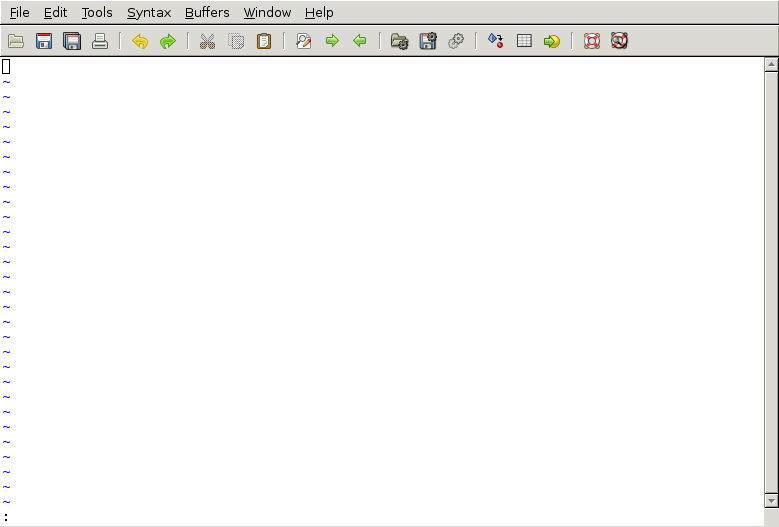
\includegraphics[width=\linewidth]{vim-new.png}
  \caption{Nouveau fichier vide.}
  \label{fig:vim-new}
\end{figure}

Commençons par entrer un commentaire dans l'en-tête du fichier pour y mentionner notre nom. Pour pouvoir entrer du texte appuyez sur \tti (le curseur devrait changer d'aspect) et entrez le commentaire ci-dessous\sidenote{Si vous ne savez pas trop ce que vous avez fait et que \vim vous affiche des trucs en rouge en bas à gauche ou ne semble pas réagir comme il faut quand vous appuyez sur \tti, appuyez plusieurs fois sur \ttesc, ça devrait vous remettre au mode par défaut de \vim}.
\begin{listing}[H]

    \begin{minted}[bgcolor=bg, gobble=8]{vim}
        " VIM Configuration - Vincent Jousse
    \end{minted}
    \caption{Votre première ligne avec \vim.}
    \label{code:first-comment}
\end{listing}

Vous aurez remarqué que les commentaires en \emph{VimL} (le langage de configuration de \vim) commencent par un \Verb|"|. Appuyez ensuite sur \ttesc pour revenir au mode par défaut (le mode normal) de \vim. Et voilà le travail, cf figure \ref{fig:vim-first-comment}.

\begin{figure}%
  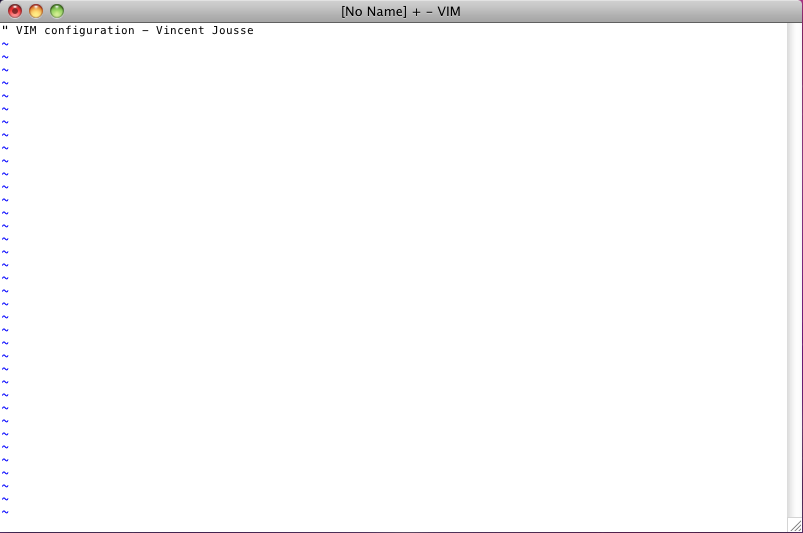
\includegraphics[width=\linewidth]{vim-first-comment.png}
  \caption{Mon premier commentaire.}
  \label{fig:vim-first-comment}
\end{figure}

Tout ça pour ça me direz-vous, et vous avez bien raison. Mais tout cela a une logique que je vais vous expliquer. L'avantage de \vim est qu'il est généralement logique. Quand vous avez compris la logique, tout vous semble limpide et tomber sous le sens.

Par défaut, \vim est lancé dans un mode que l'on appelle le mode ``Normal''. C'est à dire que ce mode n'est pas fait pour écrire du texte (ça, ça sera le mode ``Insert'') mais juste pour se déplacer et manipuler du texte. C'est la présence de ces 2 différents modes (il y en a d'autres mais ce n'est pas le sujet pour l'instant) qui fait toute la puissance de \vim. Il vous faudra un certain temps pour vous rendre compte de cette puissance par vous-même, alors faites-moi juste confiance pour l'instant.

Si vous vous demandez pourquoi ces modes, pourquoi on semble se compliquer la vie (on se la simplifie en fait) et en quel honneur, dans le mode par défaut, il n'est même pas possible d'insérer du texte, lisez attentivement la section qui suit.

\section{Les modes : d'où \vim tire sa puissance}\label{sec:modes}

Je pense que nous serons tous à peu prêt d'accord sur le fait que si vous souhaitez apprendre à utiliser \vim, c'est pour gagner en efficacité pour la saisie/manipulation de texte/code. Pour gagner en efficacité lorsque l'on tape du code il n'y a pas 36 solutions, il n'y en a qu'une en fait : il faut bouger le moins possible les mains (voire pas du tout), et ne bouger que les doigts.

Pour ce faire bien sûr, vous oubliez tout d'abord l'utilisation de la souris. En plus d'être lent, le mouvement clavier -> souris puis souris -> clavier est très mauvais pour vos articulations. Il est souvent à l'origine de troubles musculosquelettiques\sidenote{Vous êtes peut-être jeune et n'avez pas encore eu ce type de soucis. Mais croyez moi, ça vient beaucoup plus vite qu'on ne le croit. Si vous passez votre journée sur un ordinateur, ne négligez pas ces facteurs, vous le regretterez un jour.}. D'après \emph{Wikipedia}, c'est le type de maladie professionnelle la plus courante à l'heure actuelle\sidenote{\url{https://fr.wikipedia.org/wiki/Troubles_musculosquelettiques}}.

Vous oubliez aussi le mouvement de votre main droite vers les touches directionnelles gauche/droite/bas/haut. C'est une perte de temps et c'est totalement inutile avec \vim.

Qu'est-ce que vous avez le droit de faire dans le coup ? Pas grand chose, si ce n'est garder vos mains sur la position de repos comme le montre la figure \ref{fig:hand-position}. Vous trouverez d'ailleurs sur la plupart des claviers des marques sur les touches F et J, c'est pour vous donner un repère tactile de la position où doivent se trouver vos index dans la position de repos.

\begin{figure}%
  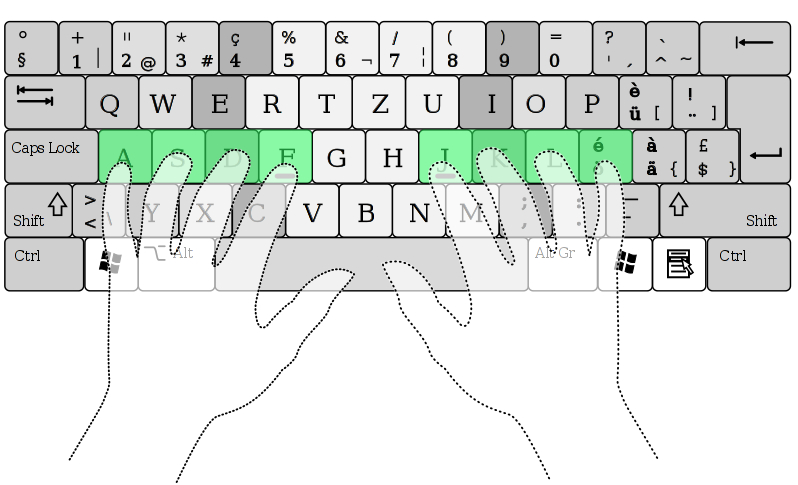
\includegraphics[width=\linewidth]{hand-position.png}
  \caption{Position de repos, clavier QWERTY. \emph{Illustration par Cy21 - CC-BY-SA-3.0 (\url{www.creativecommons.org/licenses/by-sa/3.0}) ou GFDL (\url{www.gnu.org/copyleft/fdl.html}), via Wikimedia Commons \url{http://commons.wikimedia.org/wiki/File:Typing-home-keys-hand-position.svg}}}
  \label{fig:hand-position}
\end{figure}

Ce parti pris (bouger le moins possible les mains du clavier) justifie à lui seul la présence d'un mode \emph{normal} et d'un mode \emph{insertion} dans \vim. En passant de l'un à l'autre, les touches sous vos doigts serviront tantôt à vous déplacer et à réaliser des opérations sur le texte\sidenote{C'est le mode \emph{normal}} (copier/coller, macros, \ldots), tantôt à sélectionner\sidenote{C'est le mode \emph{visuel}} et tantôt à insérer du texte\sidenote{C'est le mode \emph{insertion}}. Tout cela bien sûr en évitant l'utilisation de combinaisons de touches du style \emph{Ctrl + touche} qui ne sont généralement pas bonnes pour vos doigts (\emph{Emacs} si tu nous lis, je te salue).

Par défaut, on passe du mode \emph{insertion} au mode \emph{normal} en appuyant sur la \ttesc, mais c'est une des premières choses que l'on changera : \ttesc est bien trop loin sur les claviers actuels. 

Pour passer du mode \emph{normal} au mode \emph{insertion}, on peut par exemple appuyer sur \tti. On apprendra par la suite qu'il existe d'autres moyens de faire. Par exemple pour rentrer en mode insertion tout en créant une nouvelle ligne en dessous de la ligne courante (peu importe où se trouve votre curseur sur la ligne), on utilisera \tto en mode \emph{normal}.

J'y reviendrai plus tard dans «\nameref{sec:se-deplacer}» mais si vous n'êtes pas prêt, à terme, à ne plus utiliser votre souris et les flèches directionnelles pour éditer du texte, je vous recommande presque d'arrêter votre apprentissage maintenant, c'est aussi simple que cela. \vim révèle tout sa puissance quand il est utilisé sans souris et en bougeant le moins possible les mains.

\newthought{Si vous voulez pousser la démarche} encore plus loin, vous pouvez aussi vous procurer un clavier orthogonal \emph{TypeMatrix}\sidenote{\url{http://www.typematrix.com/}}. C'est ce que j'utilise personnellement, et mes doigts m'en remercient tous les jours.

L'ultime changement serait d'utiliser une disposition de clavier encore plus efficace comme le \emph{bépo} pour quasi doubler sa vitesse de frappe au clavier. Pour les plus curieux d'entre vous, j'explique la démarche sur mon blog : \url{http://vincent.jousse.org/comment-doubler-sa-vitesse-de-frappe-au-clavier/}.


\newpage
\section{La configuration par défaut : indispensable}

\newthought{Passons aux choses sérieuses}, c'est-à-dire comment rendre \vim un tant soit peu utilisable. Nous allons donc éditer le fichier de configuration par défaut \vimrc\sidenote{Ce fichier doit se trouver dans votre répertoire d'accueil. \emph{/home/votre\_user/.vimrc} sous Linux, \emph{/Users/votre\_user/.vimrc} sous Mac Os X ou plus généralement \emph{\textasciitilde{}/.vimrc}. Sous Windows vous pouvez créer un fichier nommé \emph{\_vimrc} qui doit se situer dans votre répertoire \emph{\%HOME\%} qui change en fonction de votre version de Windows. C'est généralement le répertoire jute "au dessus" de votre répertoire \emph{Mes Documents}. Plus d'infos sur Wikipedia \url{http://en.wikipedia.org/wiki/Home\_directory\#Default\_Home\_Directory\_per\_Operating\_System}} en y plaçant des valeurs que toute personne normalement constituée souhaiterait y voir figurer.

J'ai commenté chacune des lignes du fichier directement dans le code. Rien de sorcier ici, on se demande juste pourquoi tout cela n'est pas inclus par défaut.

\begin{listing}[H]
    \inputminted[bgcolor=bg, fontsize=\footnotesize]{vim}{../../vim-for-humans/firstconfig/vimrc}
    \caption{Une configuration par défaut sensée.}
    \label{code:first-config}
\end{listing}

J'ai mis en ligne ce fichier de configuration directement sur \emph{Github}. Vous pouvez le télécharger ou le copier directement à partir d'ici : \url{http://github.com/vjousse/vim-for-humans/fr/firstconfig/}. Il devrait aussi faire partie du package que vous avez téléchargé.

Vous devriez avoir un \vim qui ressemble à celui sur la figure \ref{fig:first-config}. Notez les numéros de ligne sur la gauche ainsi que la position du curseur en bas à droite.

\begin{figure}%
  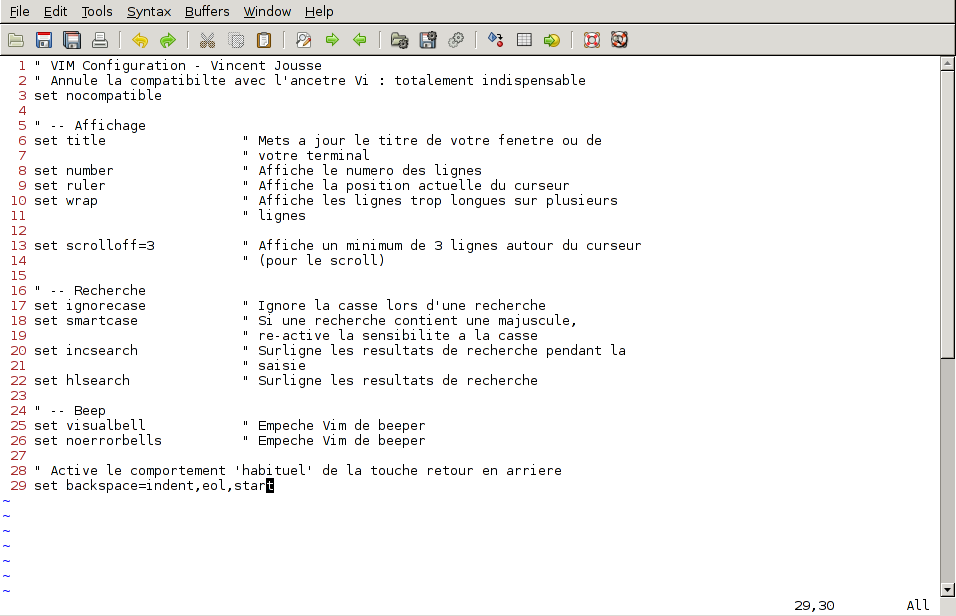
\includegraphics[width=\linewidth]{vim-first-config.png}
  \caption{\vim après votre première configuration.}
  \label{fig:first-config}
\end{figure}

Bon c'est bien beau tout ça mais ça manque un peu de couleurs. Au suivant !

\section{Que la couleur soit !}

\newthought{Tout d'abord} il faut commencer par activer la coloration syntaxique du code dans le fichier de configuration. Ajoutez ces lignes à là fin de votre fichier de configuration \vimrc.

\begin{listing}[H]
\begin{minted}[bgcolor=bg, fontsize=\footnotesize]{vim}
" Active la coloration syntaxique
syntax enable
" Active les comportements specifiques aux types de fichiers comme
" la syntaxe et l'indentation
filetype on
filetype plugin on
filetype indent on
\end{minted}
  \caption{Activation de la coloration syntaxique.}
  \label{lst:syntax-hl}
\end{listing}

Vous devriez avoir un \vim qui ressemble à celui de la figure \ref{fig:syntax-hl}\sidenote{Pour l'instant, le plus facile pour que les modifications apportées à votre \vimrc soient prises en compte, c'est de le fermer et de le ré-ouvrir. Si vous voulez vraiment vous la jouer à la \vim de suite, en mode normal tapez \vimscmd{:so \textasciitilde/.vimrc} ou \vimscmd{:so \$MYVIMRC}.

\vimscmd{:so} étant un raccourci pour \vimscmd{:source}.}. C'est une bonne première étape, passons maintenant à l'utilisation d'un thème.

\begin{figure}%
  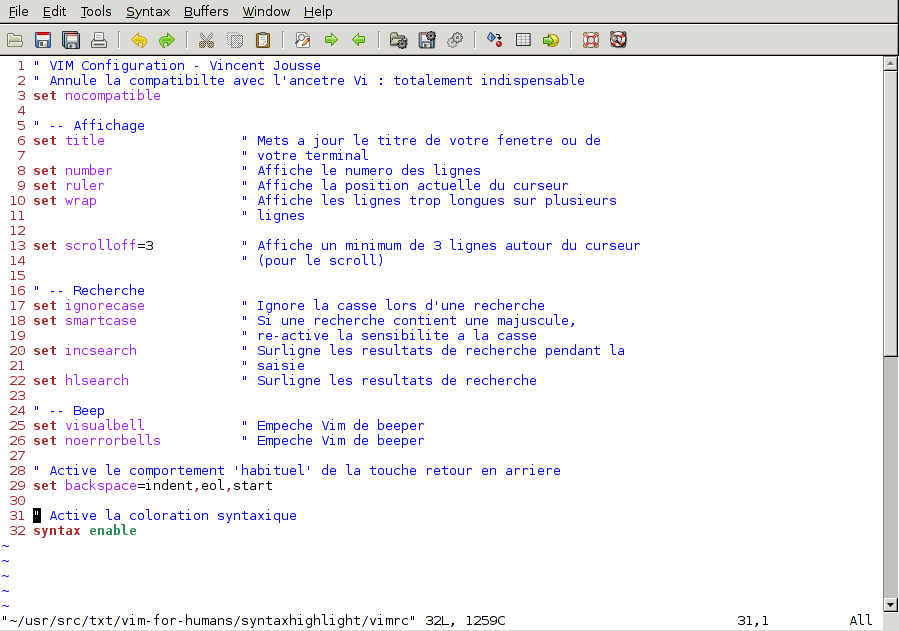
\includegraphics[width=\linewidth]{vim-syntax-hl.png}
  \caption{Coloration syntaxique par défaut.}
  \label{fig:syntax-hl}
\end{figure}

Les thèmes vont vous permettre de rendre votre \vim un peu moins austère en changeant généralement la couleur de fond ainsi que les couleurs par défaut pour le code. Comme je l'ai mentionné plus haut, nous allons utiliser le thème solarized \url{http://ethanschoonover.com/solarized} (avec fond clair ou foncé, ça dépendra de vous).

Pour l'installer, commencez tout d'abord par créer un répertoire nommé \Verb|.vim|\sidenote{Ce répertoire s'appelle \Verb|vimfiles| sous Windows. À chaque fois que je ferai référence au répertoire \Verb|.vim| ça sera en fait \Verb|vimfiles| pour les Windowsiens} au même endroit que votre \vimrc\sidenote{Dans votre répertoire utilisateur donc.}. Dans ce répertoire \Verb|.vim|, créez un sous-répertoire nommé \Verb|colors|. Téléchargez ensuite le fichier du thème Solarized \url{https://raw.github.com/altercation/vim-colors-solarized/master/colors/solarized.vim}\sidenote{ou copiez celui qui vous a été fourni avec le téléchargement de ce livre}(c'est le même fichier pour les deux versions du thème) et copiez le dans le répertoire \Verb|vim/colors/| fraîchement créé. Votre répertoire \Verb|.vim| devrait ressembler à celui de la figure \ref{fig:solarized-tree}.

\begin{figure}%
  \center
  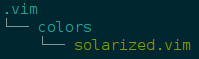
\includegraphics[width=0.3\linewidth]{solarized-tree.png}
  \caption{Le contenu du répertoire .vim avec Solarized.}
  \label{fig:solarized-tree}
\end{figure}

Activez ensuite le thème Solarized dans votre \vimrc comme le montre le code dans le listing \ref{lst:solarized}. Pour tester le thème clair, remplacez \Verb|dark| par \Verb|light| (au niveau de la définition de la propriété \Verb|background|).

\begin{listing}[H]
\begin{minted}[bgcolor=bg, fontsize=\footnotesize]{vim}
" Utilise la version sombre de Solarized
set background=dark
colorscheme solarized
\end{minted}
  \caption{Activation de la coloration syntaxique.}
  \label{lst:solarized}
\end{listing}

Les images \ref{fig:vim-solarized-dark} et \ref{fig:vim-solarized-light} vous donnent un aperçu des deux variantes (ma préférence allant à la variante sombre soit dit en re-passant).

\begin{figure}%
  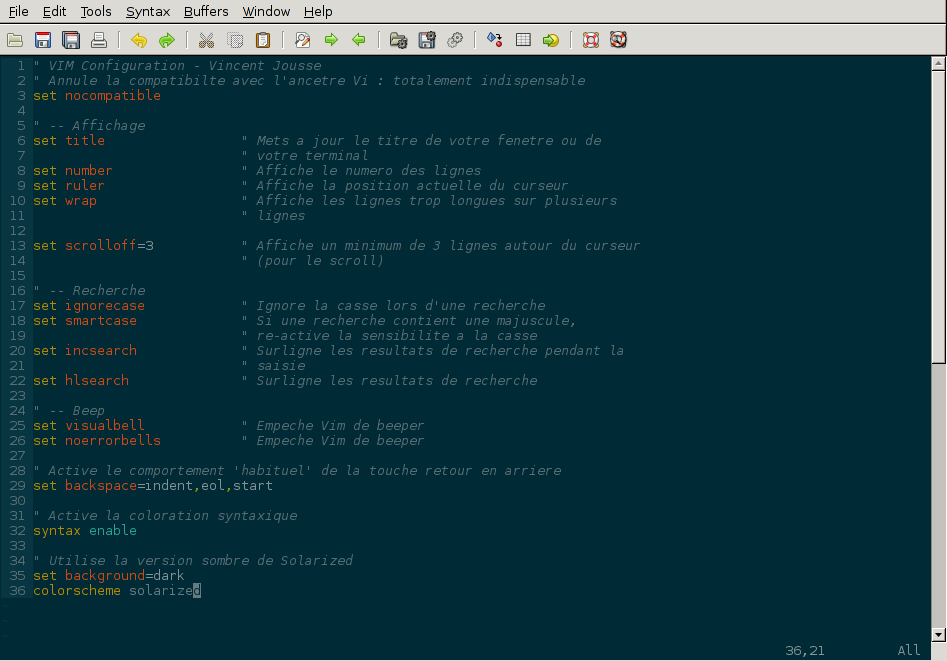
\includegraphics[width=\linewidth]{vim-solarized-dark.png}
  \caption{Le thème Solarized sombre.}
  \label{fig:vim-solarized-dark}
\end{figure}

\begin{figure}%
  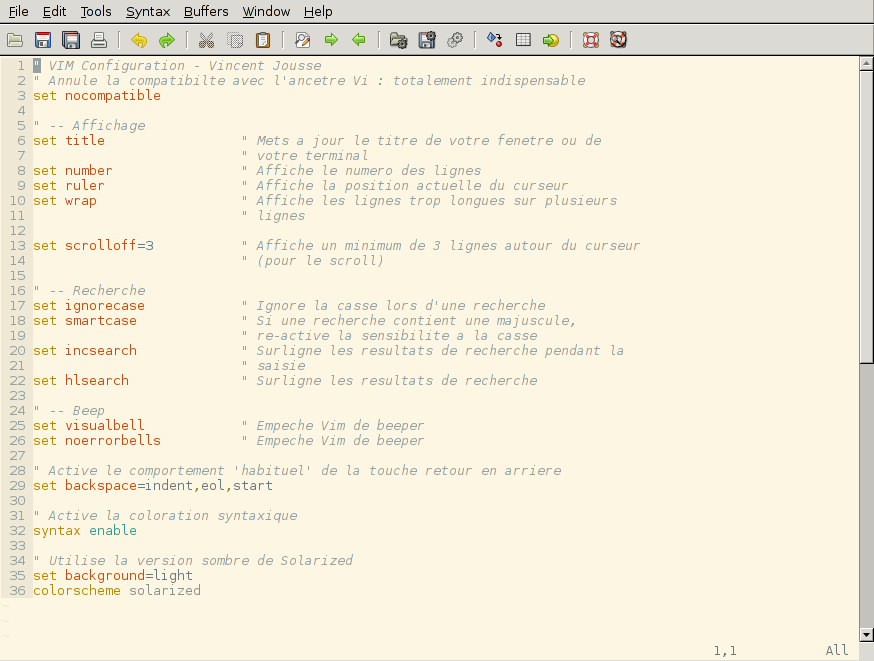
\includegraphics[width=\linewidth]{vim-solarized-light.png}
  \caption{Le thème solarized clair.}
  \label{fig:vim-solarized-light}
\end{figure}

\newthought{Un bonus} (si vous n'utilisez pas \vim directement dans votre terminal) serait de choisir une police de caractères qui vous convient un peu mieux, c'est bien sûr facultatif mais bon, je présume que certains d'entre vous sont des esthètes aguerris.

Si vous êtes sous Mac Os X je vous conseille la police \Verb|Monaco| qui est assez conviviale. Rajoutez les lignes suivantes à votre \vimrc pour l'utiliser :

\begin{listing}[H]
\begin{minted}[bgcolor=bg, fontsize=\footnotesize]{vim}
set guifont=Monaco:h13
set antialias
\end{minted}
  \caption{Utilisation de la police Monaco sous Mac Os X.}
  \label{lst:monaco}
\end{listing}

Vous pouvez bien sûr changer le \Verb|h13| par \Verb|h12| si vous voulez une police plus petite (ou par \Verb|h14| si vous en voulez une plus grande).

Sinon sous Linux j'utilise la police \Verb|DejaVu Sans Mono| que je trouve plutôt sympathique :

\begin{listing}[H]
\begin{minted}[bgcolor=bg, fontsize=\footnotesize]{vim}
set guifont=DejaVu\ Sans\ Mono\ 10
set antialias
\end{minted}
  \caption{Utilisation de la police DejaVuSansMono sous Linux.}
  \label{lst:dejavusansmono}
\end{listing}

Vous pouvez là aussi bien sûr changer la taille de la police si vous le souhaitez. Pour avoir la liste des polices disponibles tapez en mode normal \vimcmd{:set guifont:*}.

Vous trouverez une version complète du fichier de configuration pour ce chapitre en ligne \url{https://github.com/vjousse/vim-for-humans/blob/master/syntaxhighlight/vimrc} ou avec les fichiers mis à disposition avec ce livre. Je ne m'attarderai pas plus sur les polices, c'est assez dépendant de votre système d'exploitation, et un peu moins de \vim dans le coup.


\section{L'explorateur de fichiers : notre premier plugin}

Nous y voilà, nous avons un \vim à peu près utilisable avec de jolies couleurs. Maintenant, il faudrait être capable d'ouvrir des fichiers autrement qu'en faisant \Verb|Fichier (File) -> Ouvrir (Open)|. Ça va être une bonne occasion pour installer notre premier plugin (ce n'est pas comme si nous avions d'autres choix de toute façon). Nous allons procéder ici en deux étapes, tout d'abord installer un gestionnaire de plugins pour éviter que ça devienne trop le bazar dans vos plugins, puis installer ensuite le plugin qu'il nous faut pour explorer un répertoire de fichiers.

\subsection{Gestionnaire de plugins: Pathogen}

Pathogen\sidenote{\url{https://github.com/tpope/vim-pathogen/}} est typique du plugin que vous découvrez après avoir commencé à configurer votre \vim et qui génère ce type de réaction : "Ah si j'avais su j'aurais directement commencé avec". Ça tombe bien, c'est ce que nous allons faire.

Tout d'abord, petite explication de comment on installe et configure des plugins dans \vim. Ils s'installent en copiant les fichiers adéquats (la plupart du temps avec une extension en \emph{*.vim}) dans des sous-répertoires de votre répertoire de configuration \emph{.vim}. On a déjà d'ailleurs commencé à y créer un sous-répertoire \Verb|colors| qui contient notre "plugin" de coloration Solarized.

Le problème avec cette approche c'est que les différents plugins ne sont pas isolés (vous allez devoir copier leurs fichiers dans les différents sous-répertoires) et que vous allez donc vous retrouver avec des fichiers un peu partout sans savoir à qui ils appartiennent. Autant vous dire qu'une fois que vous voulez désinstaller ou mettre à jour un plugin, c'est vite l'enfer pour savoir quels sont ses fichiers.

C'est là que pathogen arrive à la rescousse, il va vous permettre d'installer chaque plugin dans un sous-répertoire rien que pour lui. La figure \ref{fig:pathogen-tree} vous donne un exemple de répertoire \Verb|.vim| avant et après l'utilisation de pathogen. Certes la version avec pathogen contient plus de sous-répertoires, mais croyez-moi sur parole, ce rangement va vous éviter bien des ennuis par la suite\sidenote{Et vous pourrez au passage très facilement utiliser \emph{git} pour gérer chacun de vos plugins comme des submodules, ce qu'il est impossible de réaliser sinon.}.

\begin{figure}%
  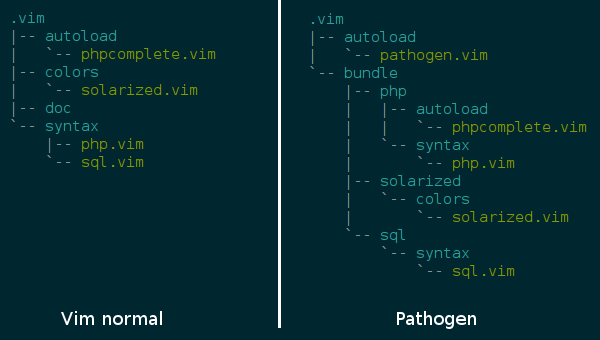
\includegraphics[width=\linewidth]{pathogen-tree.png}
  \caption{\emph{.vim} avant et après Pathogen.}
  \label{fig:pathogen-tree}
\end{figure}

Commençons par installer pathogen. Créez un répertoire nommé \Verb|autoload| dans votre répertoire \Verb|.vim| et copiez y \Verb|pathogen.vim| que vous pouvez télécharger ici : \url{https://raw.github.com/tpope/vim-pathogen/master/autoload/pathogen.vim} (ou qui vous a été fourni avec ce PDF). Pour les utilisateurs Unix, le listing \ref{code:pathogen-install} explique comment l'installer\sidenote{Si vous n'avez pas \Verb|{\footnotesize curl}| vous pouvez aussi utiliser \scmd{wget -O -}}.

\begin{listing}[H]
\begin{minted}[bgcolor=bg, fontsize=\footnotesize]{sh}
# Creation du repertoire autoload
mkdir -p ~/.vim/autoload 

# Telechargement et installation de pathogen
curl -so ~/.vim/autoload/pathogen.vim \
    https://raw.github.com/tpope/vim-pathogen/master/autoload/pathogen.vim
\end{minted}
  \caption{Installation de pathogen.}
  \label{code:pathogen-install}
\end{listing}

Nous installerons ensuite nos plugins directement dans le répertoire \Verb|.vim/bundle| que vous allez vous empresser de créer, cf. le listing \ref{code:pathogen-bundle}.

\begin{listing}[H]
\begin{minted}[bgcolor=bg, fontsize=\footnotesize]{sh}
# Creation du repertoire bundle
mkdir -p ~/.vim/bundle
\end{minted}
  \caption{Création du répertoire d'installation des plugins.}
  \label{code:pathogen-bundle}
\end{listing}

Il ne vous reste plus qu'à activer pathogen dans votre \vimrc et le tour est joué. Nous placerons le code listé dans 
\ref{code:pathogen} au début du fichier \vimrc, directement après la ligne \Verb|set nocompatible|.

\begin{listing}[H]

\begin{minted}[bgcolor=bg]{vim}
" Activation de pathogen
call pathogen#infect()
\end{minted}
\caption{Activation du plugin pathogen.}
\label{code:pathogen}
\end{listing}

Puisque charité bien ordonnée commence par soi-même, nous allons ranger notre petit plugin solarized en utilisant pathogen. Il nous suffit de créer un répertoire \Verb|solarized| dans notre répertoire \Verb|bundle| fraîchement créé\sidenote{Vous pouvez l'appeler comme vous le souhaitez, tout sous-répertoire du répertoire \Verb|{\footnotesize bundle}| sera considéré comme un répertoire de plugin.}. Nous déplaçons ensuite le répertoire \Verb|colors| dans le répertoire \Verb|solarized| (cf. le listing \ref{code:solarized-bundle}).

\begin{listing}[H]
\begin{minted}[bgcolor=bg, fontsize=\footnotesize]{sh}
# Creation du repertoire pour solarized
mkdir ~/.vim/bundle/solarized
# Et hop un peu de rangement
mv ~/.vim/colors ~/.vim/bundle/solarized
\end{minted}
  \caption{Utilisation de solarized via pathogen.}
  \label{code:solarized-bundle}
\end{listing}

Actuellement, Pathogen reste encore le gestionnaire de plugins \vim le plus utilisé. Mais depuis peu, un challenger est arrivé, il s'appelle Vundle \url{https://github.com/gmarik/vundle}. J'ai choisi de vous présenter Pathogen car c'est de lui que vous entendrez parler le plus, mais sachez que Vundle est aussi une alternative intéressante : il est compatible avec Pathogen et il gère les versions et les mises à jours de vos plugins directement depuis internet. Pour ceux qui connaissent Ruby, c'est le Bundler \sidenote{\url{http://gembundler.com/}} pour \vim.


Voilà notre \vim est presque près pour le grand bain. Il vous reste une petite étape à franchir : disposer d'un moyen pratique pour explorer les fichiers d'un projet, c'est ici que \emph{The NERD Tree} entre en lice.

\subsection{Explorateur de fichiers : The NERD Tree}
\label{ssec:nerdtree}
The NERD Tree est un plugin permettant d'afficher visuellement une arborescence de fichiers directement dans la partie gauche (par défaut) de votre \vim, à la \emph{TextMate}, \emph{Sublime Text} ou encore \emph{Eclipse/Netbeans}. Ce plugin n'est pas essentiel si vous souhaitez tout contrôler au clavier (je ne l'utilise plus moi-même), mais est assez pratique lorsque l'on débute avec \vim.

L'alternative que nous verrons plus tard au chapitre \TODO est d'utiliser les plugin \emph{Ctrl-p} ou \emph{Command-t} pour trouver des fichiers et les plugins \emph{LustyExplorer} et \emph{LustyJuggler} pour naviguer entre les fichiers. En effet, devoir visualiser l'arborescence pour trouver un fichier est toujours plus lent que de trouver le fichier à partir de son nom par exemple. The NERD Tree vous permettra donc d'obtenir un \vim se comportant comme un éditeur classique avec un explorateur de fichiers sur lequel vous pourrez cliquer.

Nous allons tout d'abord préparer pathogen pour installer les différents fichiers de \emph{The NERD Tree}.

\begin{listing}[H]
\begin{minted}[bgcolor=bg, fontsize=\footnotesize]{sh}
# Creation du repertoire pour The NERD Tree
mkdir ~/.vim/bundle/nerdtree
\end{minted}
  \caption{Création du répertoire pour The NERD Tree.}
  \label{code:nerdtree-bundle}
\end{listing}

Téléchargez ensuite le dernier \emph{.zip} disponible sur la page du plugin \url{http://www.vim.org/scripts/script.php?script_id=1658}. À l'heure où j'écris ces lignes la dernière version disponible est la version 4.2.0 disponible en téléchargement à cette adresse\sidenote{C'est la version que vous trouverez dans les fichiers mis à disposition avec ce PDF} : \url{http://www.vim.org/scripts/download_script.php?src_id=17123}.

Ouvrez le fichier zip et placez son contenu dans le répertoire \Verb|~/.vim/bundle/nerdtree| que nous venons de créer. Vous devriez avoir une arborescence ressemblant à celle ci-dessous pour votre répertoire \Verb|nerdtree| :

\begin{verbatim}
nerdtree
|-- doc
|   `-- NERD_tree.txt
|-- nerdtree_plugin
|   |-- exec_menuitem.vim
|   `-- fs_menu.vim
|-- plugin
|   `-- NERD_tree.vim
`-- syntax
    `-- nerdtree.vim
\end{verbatim}

Il va ensuite falloir activer le plugin. Vous pouvez le faire manuellement en tapant \vimcmd{:NERDTree} en mode normal. Si vous préférez activer \emph{The NERD Tree} à chaque fois que vous ouvrez votre \vim, ajoutez ces lignes dans votre \vimrc:

\begin{listing}[H]
\begin{minted}[bgcolor=bg]{vim}
" Activation de NERDTree au lancement de vim
autocmd vimenter * NERDTree
\end{minted}
\caption{Activation de NERDTree au lancement de \vim.}
\label{code:nerdtreee}
\end{listing}

Rien de particulier ensuite, \emph{The NERD Tree} vous affiche l'arborescence du répertoire où vous avez lancé \vim, comme vous le montre la figure \ref{fig:vim-nerdtree}. Vous pouvez utiliser la souris et/ou le clavier pour vous déplacer. 

Vous pouvez aussi effectuer des commandes (créer, copier des fichiers) en appuyant sur \ttm lorsque vous êtes dans \emph{The NERD Tree}. Pour passer de la fenêtre de \emph{NERD Tree} à la fenêtre d'édition de votre fichier au clavier, appuyez sur \hlred{Ctrl + w} puis \hlred{w}\sidenote{La touche \hlred{\emph{Control}} (Ctrl) et tout en la laissant appuyée la touche \hlred{w}. Vous pouvez ensuite tout lâcher pour appuyer une nouvelle fois sur \hlred{w}.}. Ce raccourci clavier sera d'ailleurs toujours valable pour naviguer entre vos différentes fenêtres \vim (il n'est pas spécifique à \emph{The NERD Tree}).

\begin{figure}%
  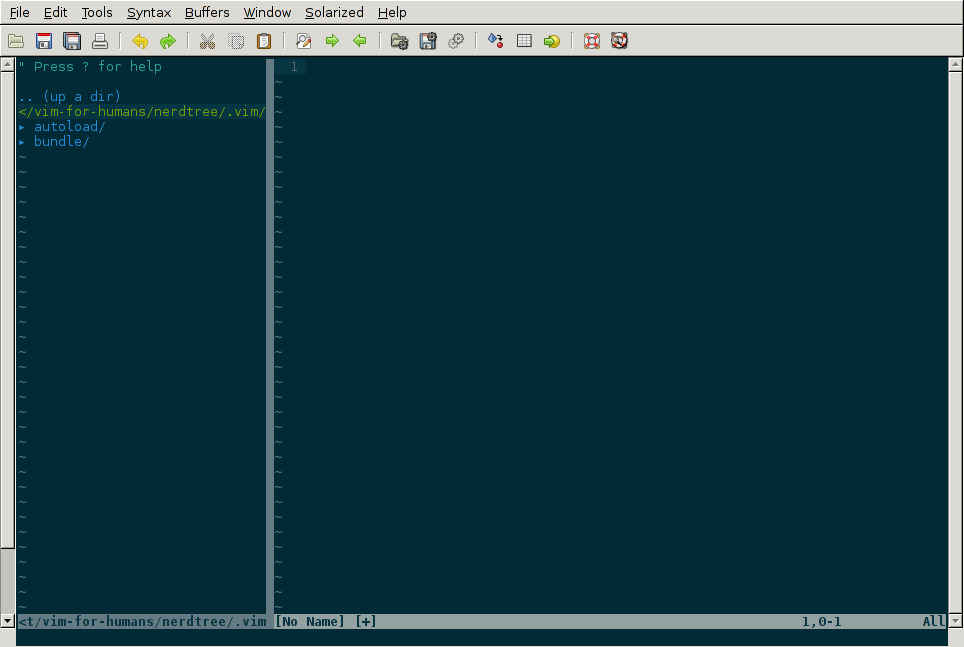
\includegraphics[width=\linewidth]{vim-nerdtree.png}
  \caption{\emph{.vim} avec \emph{The NERD Tree} d'activé.}
  \label{fig:vim-nerdtree}
\end{figure}

\section{Nous voilà fin prêts}

Nous venons de couvrir ce qui pour moi manque cruellement à \vim : une configuration par défaut acceptable. Je ne dis pas que c'est la panacée pour l'instant, mais ça devrait vous permettre d'avoir un \vim utilisable comme n'importe quel autre éditeur de texte dont vous ne connaissez pas encore toutes les possibilités. Vous pouvez pour l'instant utiliser la souris pour faire un peu tout ce que vous voulez, heureusement ça ne va pas durer.

Nous allons maintenant aborder ce qui fait que \vim est unique et tant prisé : sa gestion des modes et des commandes pour manipuler le texte. La balle est dans votre camp maintenant : ou vous êtes prêt à changer vos habitudes et à passer à un autre niveau d'efficacité, ou alors n'utiliser \vim que comme un bloc-notes amélioré vous convient\footnote{Dans ce cas là, vous pouvez vous arrêter là.}. C'est vous qui voyez !
